% Options for packages loaded elsewhere
\PassOptionsToPackage{unicode}{hyperref}
\PassOptionsToPackage{hyphens}{url}
%
\documentclass[
]{book}
\usepackage{amsmath,amssymb}
\usepackage{lmodern}
\usepackage{iftex}
\ifPDFTeX
  \usepackage[T1]{fontenc}
  \usepackage[utf8]{inputenc}
  \usepackage{textcomp} % provide euro and other symbols
\else % if luatex or xetex
  \usepackage{unicode-math}
  \defaultfontfeatures{Scale=MatchLowercase}
  \defaultfontfeatures[\rmfamily]{Ligatures=TeX,Scale=1}
\fi
% Use upquote if available, for straight quotes in verbatim environments
\IfFileExists{upquote.sty}{\usepackage{upquote}}{}
\IfFileExists{microtype.sty}{% use microtype if available
  \usepackage[]{microtype}
  \UseMicrotypeSet[protrusion]{basicmath} % disable protrusion for tt fonts
}{}
\makeatletter
\@ifundefined{KOMAClassName}{% if non-KOMA class
  \IfFileExists{parskip.sty}{%
    \usepackage{parskip}
  }{% else
    \setlength{\parindent}{0pt}
    \setlength{\parskip}{6pt plus 2pt minus 1pt}}
}{% if KOMA class
  \KOMAoptions{parskip=half}}
\makeatother
\usepackage{xcolor}
\IfFileExists{xurl.sty}{\usepackage{xurl}}{} % add URL line breaks if available
\IfFileExists{bookmark.sty}{\usepackage{bookmark}}{\usepackage{hyperref}}
\hypersetup{
  pdftitle={projectname: Developing the Evidence Base: Final Project Report ~\textbackslash{}},
  pdfauthor={Simon Knight},
  hidelinks,
  pdfcreator={LaTeX via pandoc}}
\urlstyle{same} % disable monospaced font for URLs
\usepackage{longtable,booktabs,array}
\usepackage{calc} % for calculating minipage widths
% Correct order of tables after \paragraph or \subparagraph
\usepackage{etoolbox}
\makeatletter
\patchcmd\longtable{\par}{\if@noskipsec\mbox{}\fi\par}{}{}
\makeatother
% Allow footnotes in longtable head/foot
\IfFileExists{footnotehyper.sty}{\usepackage{footnotehyper}}{\usepackage{footnote}}
\makesavenoteenv{longtable}
\usepackage{graphicx}
\makeatletter
\def\maxwidth{\ifdim\Gin@nat@width>\linewidth\linewidth\else\Gin@nat@width\fi}
\def\maxheight{\ifdim\Gin@nat@height>\textheight\textheight\else\Gin@nat@height\fi}
\makeatother
% Scale images if necessary, so that they will not overflow the page
% margins by default, and it is still possible to overwrite the defaults
% using explicit options in \includegraphics[width, height, ...]{}
\setkeys{Gin}{width=\maxwidth,height=\maxheight,keepaspectratio}
% Set default figure placement to htbp
\makeatletter
\def\fps@figure{htbp}
\makeatother
\setlength{\emergencystretch}{3em} % prevent overfull lines
\providecommand{\tightlist}{%
  \setlength{\itemsep}{0pt}\setlength{\parskip}{0pt}}
\setcounter{secnumdepth}{5}
\newlength{\cslhangindent}
\setlength{\cslhangindent}{1.5em}
\newlength{\csllabelwidth}
\setlength{\csllabelwidth}{3em}
\newlength{\cslentryspacingunit} % times entry-spacing
\setlength{\cslentryspacingunit}{\parskip}
\newenvironment{CSLReferences}[2] % #1 hanging-ident, #2 entry spacing
 {% don't indent paragraphs
  \setlength{\parindent}{0pt}
  % turn on hanging indent if param 1 is 1
  \ifodd #1
  \let\oldpar\par
  \def\par{\hangindent=\cslhangindent\oldpar}
  \fi
  % set entry spacing
  \setlength{\parskip}{#2\cslentryspacingunit}
 }%
 {}
\usepackage{calc}
\newcommand{\CSLBlock}[1]{#1\hfill\break}
\newcommand{\CSLLeftMargin}[1]{\parbox[t]{\csllabelwidth}{#1}}
\newcommand{\CSLRightInline}[1]{\parbox[t]{\linewidth - \csllabelwidth}{#1}\break}
\newcommand{\CSLIndent}[1]{\hspace{\cslhangindent}#1}
\usepackage{booktabs}
\usepackage{pdfpages}
\usepackage{amsthm}
\makeatletter
\def\thm@space@setup{%
  \thm@preskip=8pt plus 2pt minus 4pt
  \thm@postskip=\thm@preskip
}
\makeatother
\let\oldmaketitle\maketitle
\AtBeginDocument{\let\maketitle\relax}
\usepackage{xcolor}
\usepackage{titling}
\usepackage{pdfpages}
\usepackage{fancyhdr}
\usepackage{floatrow}
\usepackage{caption}
\definecolor{bluerich}{RGB}{13,65,209}
\usepackage{titling}
\pretitle{\begin{center}
\floatsetup[figure]{capposition=top}

\includegraphics[width=2in,height=2in]{data/00-misc/logo.png}\LARGE\\}
\posttitle{\end{center}}
\setlength{\headheight}{23pt}
\addtolength{\topmargin}{-11pt}
\fancyfoot[L]{\footnotesize\textcolor{bluerich}{\textbf{University of Technology Sydney} \\ Centre for Research on Education in a Digital Society (CREDS) \\ TD School}}
\fancyfoot[C]{\thepage}
\renewcommand{\footrulewidth}{2pt}
\fancyhead[L]{\itshape\nouppercase{\rightmark}}
\fancyhead[R]{Section \arabic{chapter}}
\pagestyle{fancy}
\ifLuaTeX
  \usepackage{selnolig}  % disable illegal ligatures
\fi

\title{projectname: Developing the Evidence Base: Final Project Report ~\textbackslash{}}
\usepackage{etoolbox}
\makeatletter
\providecommand{\subtitle}[1]{% add subtitle to \maketitle
  \apptocmd{\@title}{\par {\large #1 \par}}{}{}
}
\makeatother
\subtitle{Knight, S., (2022). projectname: Developing the Evidence Base -- Final Project Report. University of Technology Sydney.}
\author{Simon Knight}
\date{2022-07-25}

\begin{document}
\maketitle

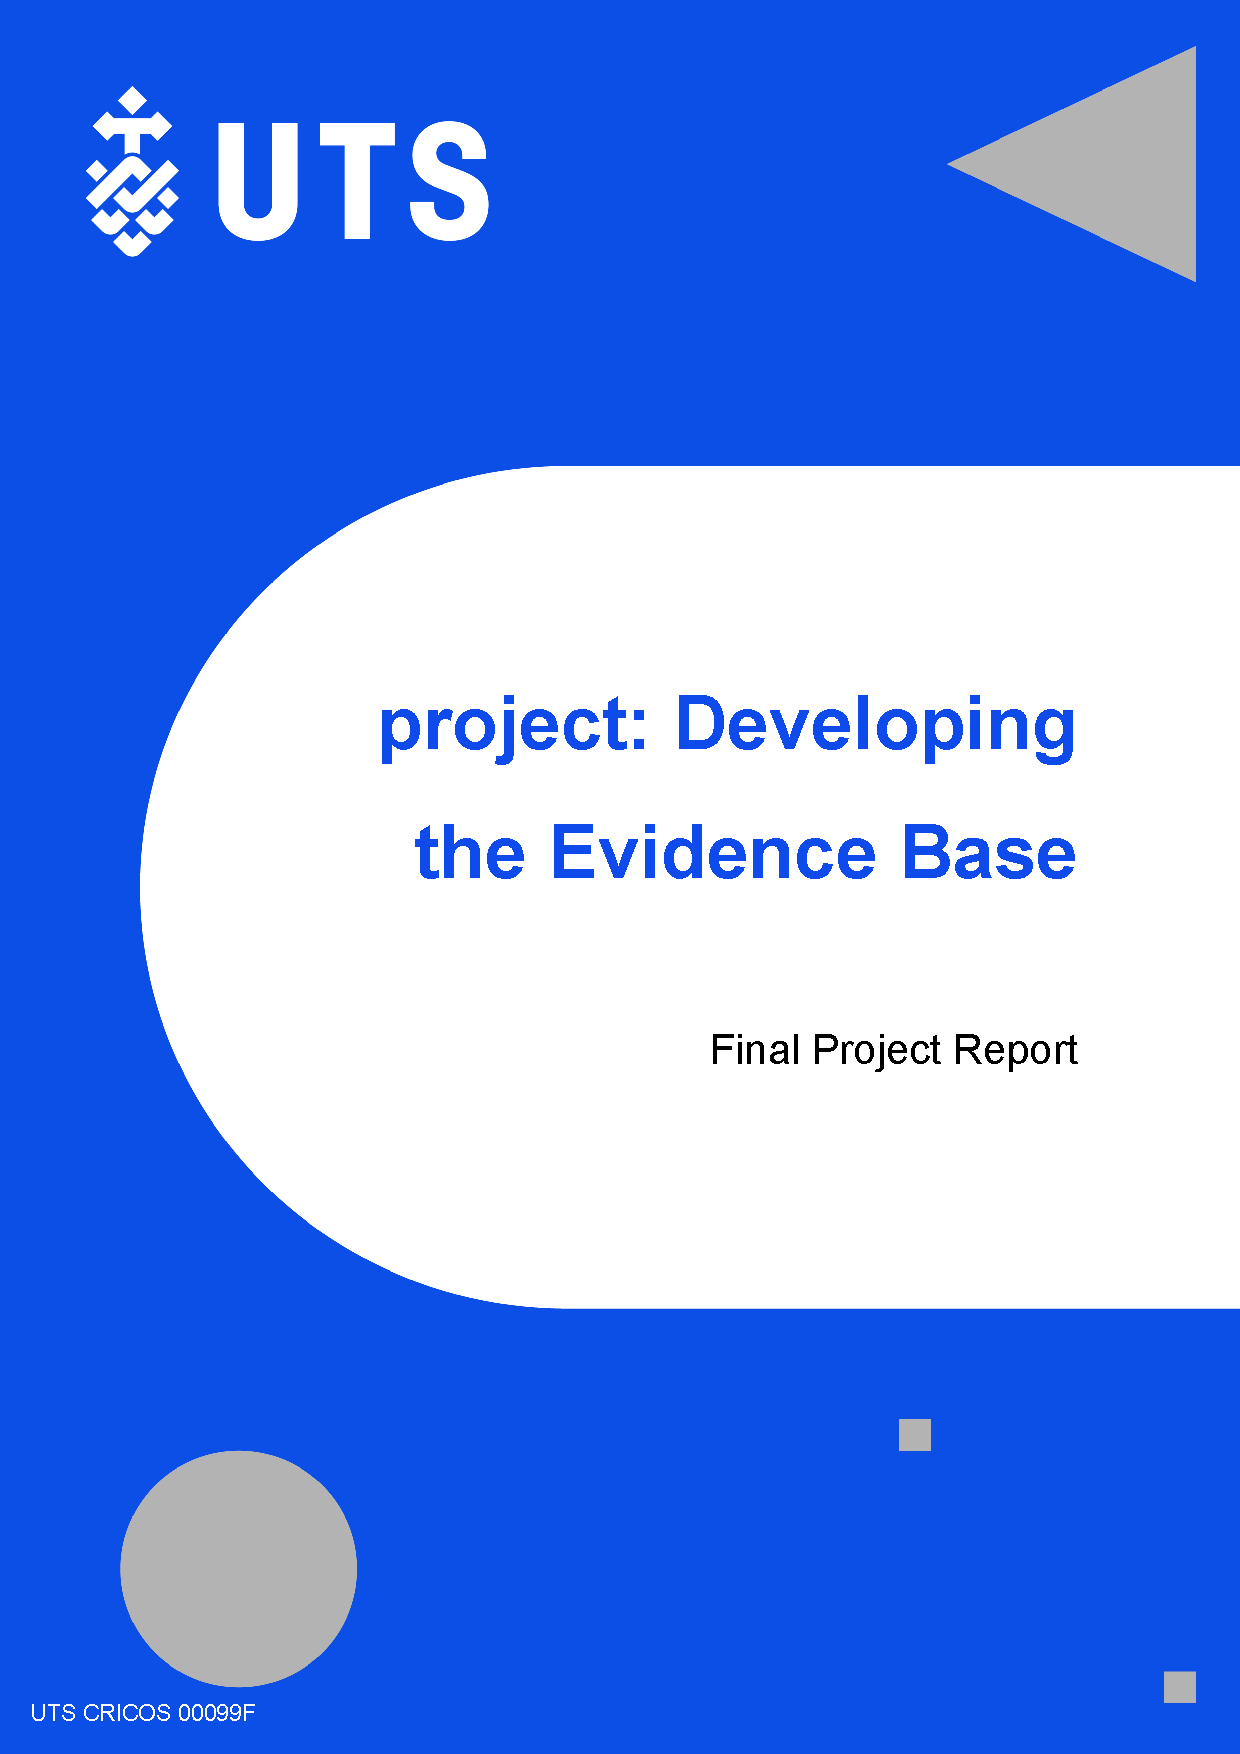
\includepdf[pages={1,2}, scale=1]{data/00-misc/00_Cover.pdf}
\newpage

\let\maketitle\oldmaketitle
\maketitle

{
\setcounter{tocdepth}{1}
\tableofcontents
}
\hypertarget{working-with-this-document}{%
\chapter{Working with this document}\label{working-with-this-document}}

This report was written as a wrapper site to compile a set of outputs, along with their rationale and the overarching narrative. It was written using a tool called \emph{bookdown}, with the aim to make it easier to navigate the materials without getting lost (and to support export to other formats like PDF).

This dummy demonstates two key things:

\begin{enumerate}
\def\labelenumi{\arabic{enumi}.}
\tightlist
\item
  The - very messy - rureporting package, primarily the function \texttt{include\_doc} which will either iframe embed documents (pptx, docx, pdf - all converted to pdf); or merge docs into a single PDF; a function \texttt{include\_frag} will take a docx and convert to markdown for inclusion in the html.
\item
  Show how the files were setup\ldots it's quite messy, but without playing more with \texttt{LaTeX} it broadly let me do the things I wanted to in terms of combining documents in a smarter way than Word allowed
\end{enumerate}

Feel free to adapt bits (please credit me if it's useful), obviously the colour scheme and branding are linked to my current institution and cannot be used.

\hypertarget{intro}{%
\chapter{Introduction}\label{intro}}

\hypertarget{about-the-research}{%
\section{About the research}\label{about-the-research}}

The project proceeded as described in the project proposal below. This report provides a compilation of the outputs created through the research, and how these contribute to the intended outcomes.

The work was executed with the following scope and context, that the research would:

\begin{itemize}
\tightlist
\item
  key context 1
\item
  key scope 2
\item
  key scope 3 consider alignment of proposals with respect to the tool as it is, to ensure any recommendations were relatively agnostic with respect to the tool design (unless evidence based rationales existed)
\end{itemize}

The research aimed to develop resources that would:

\begin{enumerate}
\def\labelenumi{\arabic{enumi}.}
\tightlist
\item
  ground the tool in evidence, with an aim to (a) maximise efficacy, and (b) provide materials and a model to communicate this evidence to stakeholders;
\item
  provide a path for ongoing research and evaluation; and
\item
  develop resources to be incorporated into the tool
\end{enumerate}

This was set out in a (lightly updated) project plan, as in \ref{fig:final-proposal}.

\hypertarget{project-plan}{%
\section{Project plan}\label{project-plan}}


\includepdf[pages=-,noautoscale, width=205mm, height = 240mm, pagecommand={}]{data/00-misc/01-2021-06-21-Final-Proposal.pdf}\label{fig:final-proposal}

\hypertarget{overview}{%
\chapter{Overview of Research Outcomes}\label{overview}}

\hypertarget{overview-of-project-and-outcomes}{%
\section{Overview of project and outcomes}\label{overview-of-project-and-outcomes}}

The research was conducted through a collaborative project between \ldots.

UTS undertook:

\begin{itemize}
\tightlist
\item
  A mapping activity to identify the program logic and theory of change for the platform (see \ref{model} ).
\item
  Evidence synthesis, targeting the key drivers in the model, distiling this evidence into key recommendations, and stakeholder-oriented FAQ (see \ref{evidence-synthesis} )
\item
  Evidence synthesis and design mapping, drawing on existing resources and evidence to develop practical resources for the intervention\ldots{}
\item
  User research, using scenarios that helped focus the evidence synthesis and connect user experience to key issues in design and development (see \ref{users} )
\end{itemize}

\hypertarget{overview-of-resources-produced}{%
\subsection{Overview of resources produced}\label{overview-of-resources-produced}}

Practically, this work has produced:

\begin{itemize}
\tightlist
\item
  A theory of change via a feature:outcome matrix model, with key questions and drivers identified
\item
  Evidence syntheses * 3

  \begin{itemize}
  \tightlist
  \item
    FAQ distillations * 3
  \end{itemize}
\item
  An overview of models\ldots{}
\item
  An overview of intervention models and theories of behaviour change, with implications for \ldots{}
\item
  A classroom slidedeck, and teacher resources to support stakeholder understanding of, and engagement with the tool
\item
  An approach to mapping resources for use in the tool, and a preliminary mapping of these into an xslx
\item
  A user study with key user insights and connections of this to the existing evidence base
\end{itemize}

\hypertarget{model}{%
\chapter{Mapping theory of change through a feature:output matrix}\label{model}}

\hypertarget{brief-background-to-theory-of-change}{%
\section{Brief background to theory of change}\label{brief-background-to-theory-of-change}}

Theories of change can be used to make clear how learning technology
innovations are designed to produce their desired outcomes in a given
context (Century \& Cassata, 2016; Cukurova et al., 2019; Weatherby et
al., 2022).

However, identifying the key features in technologies that produce their
impact can be hard. Therefore, working with a range of experts and end
users, with the technology and resources created to support the
innovation, can be a helpful way to identify and define these features,
and express their relationship to outcomes (Century \& Cassata, 2016).

It can also be challenging to align research evidence with innovations
and existing practices, because priorities in evidence production and
use may differ, and often we have to navigate incomplete or jigsawed
evidence alongside new and emerging tools and practices (Ming \&
Goldenberg, 2021, p.~130). For example, while evidence is often referred
to in terms of a hierarchy from anecdotal to causal (often randomised
control trials), this may not reflect evidence \emph{quality} for particular
\emph{purposes} (Cukurova et al., 2019; Weatherby et al., 2022)\emph{.}

Similar to logic models, in the field of `persuasive technology'
behaviour change support systems can be modelled using an
`outcome/change' design matrix. These matrices are intended to map
desired changes (attitudes, existing behaviours, or compliance with new
behaviours), to outcome spaces (formation, alternation, reinforcement)
(Langrial et al., 2013; Tikka \& Oinas-Kukkonen, 2019). This model can be
used to map \emph{features} that target particular behavioural or attitudinal
changes, to \emph{outcomes} that reflect the longer term changes in users.
Moreover, they provide an additional approach to mapping evidence to
connect features of interventions to desired outcomes.

Similarly, `driver diagrams' have been used in implementation and
improvement research in education, to express how the key drivers
towards our goals are addressed by secondary-drivers, to develop
measurement models that allow us to test interventions across contexts
(Bryk et al., 2015).

Practically, many funders now \emph{require} applicants to have an explicit
theory of change model. For example, the Victorian government `Mental
Health Fund and Menu' supplier application requires a logic model. These
can be used to:

\begin{enumerate}
\def\labelenumi{\arabic{enumi}.}
\item
  Make explicit how tools/interventions are connected to existing
  evidence
\item
  Shape product development, by making clear how proposed product
  changes influence desired outcomes
\item
  Drive evaluation by clearly defining desired outcomes, the
  observable indicators and outputs we may measure to evaluate
  progress on these outcomes, and the features of the tool that may be
  producing outcomes (and could be systematically varied).
\end{enumerate}

\hypertarget{references-in-this-section}{%
\section{References in this section}\label{references-in-this-section}}

Bryk, A. S., Gomez, L. M., Grunow, A., \& LeMahieu, P. G. (2015).
\emph{Learning to improve: How America's schools can get better at getting
better}. Harvard Education Press.

Century, J., \& Cassata, A. (2016). Implementation Research: Finding
Common Ground on What, How, Why, Where, and Who. \emph{Review of Research in
Education}, \emph{40}(1), 169--215. \url{https://doi.org/10.3102/0091732X16665332}

Cukurova, M., Luckin, R., \& Clark-Wilson, A. (2019). Creating the golden
triangle of evidence-informed education technology with EDUCATE.
\emph{British Journal of Educational Technology}, \emph{50}(2), 490--504.
\url{https://doi.org/10.1111/bjet.12727}

Langrial, S., Stibe, A., \& Oinas-Kukkonen, H. (2013). Practical Examples
of Mobile and Social Apps using the Outcome/Change Design Matrix.
\emph{PERSUASIVE (Adjunct Proceedings)}, 7--13.

Ming, N. C., \& Goldenberg, L. B. (2021). Research Worth Using:
(Re)Framing Research Evidence Quality for Educational Policymaking and
Practice. \emph{Review of Research in Education}, \emph{45}(1), 129--169.
\url{https://doi.org/10.3102/0091732X21990620}

Tikka, P., \& Oinas-Kukkonen, H. (2019). Tailoring persuasive technology:
A systematic review of literature of self-schema theory and
transformative learning theory in persuasive technology context.
\emph{Cyberpsychology: Journal of Psychosocial Research on Cyberspace},
\emph{13}(3), Article 3. \url{https://doi.org/10.5817/CP2019-3-6}

Weatherby, K., Clark-Wilson, A., Cukurova, M., \& Luckin, R. (2022). The
Importance of Boundary Objects in Industry-Academia Collaborations to
Support Evidencing the Efficacy of Educational Technology. \emph{TechTrends},
1--14.

\hypertarget{the-model}{%
\section{The model}\label{the-model}}

UTS and x have co-developed a model that represents x's program logic, and allows mapping to evidence and evaluation against this logic. The model is based on:

\begin{enumerate}
\def\labelenumi{\arabic{enumi}.}
\tightlist
\item
  Our discussions and x's existing stated model (grounded in practice and experience)
\item
  Consultation with subject matter expertise
\item
  Our knowledge and initial scan of the literature and relevant policy and practices resources
\end{enumerate}

This representation of the model shows how x's key features relate to its key outcomes and drivers. It was used to create key questions, targeted in the evidence synthesis and user testing, as shown in \ref{fig:model}. The aim of this model was to focus on the key grounding evidence, and where that evidence might have implications for change and evaluation models

\hypertarget{the-model-1}{%
\subsection{The model}\label{the-model-1}}


\includepdf[pages=-,noautoscale, width=205mm, height = 240mm, pagecommand={}]{data/03-model/03-model-v3.pdf}\label{fig:model}

\hypertarget{adaptability-to-program-logic-models}{%
\subsection{Adaptability to program logic models}\label{adaptability-to-program-logic-models}}

This model is intended to be adaptable to a traditional logic model, as in the example (removed here)

\hypertarget{evidence-synthesis}{%
\chapter{Evidence synthesis: Situating + directions for evaluation and development}\label{evidence-synthesis}}

We have developed a synthesis of evidence, based on the program logic matrix \ref{model} and questions. These syntheses should:

\begin{itemize}
\tightlist
\item
  Represent the evidence base x draws on and give language to that
\item
  Be shareable providing stakeholders with an understanding of the research background
\item
  Support development of x by pointing to gaps (in the tool, or existing evidence) and methods for evaluation
\end{itemize}

In each of the syntheses, the sections and purposes should:

\begin{itemize}
\tightlist
\item
  Provide a key summary
\item
  Highlight implications\\
\item
  Point to lessons for future work
\item
  Link to practical use cases (including those expressed in the developed scenarios).
\end{itemize}

These resources comprise:

\begin{enumerate}
\def\labelenumi{\arabic{enumi}.}
\tightlist
\item
  {Three evidence syntheses }.
\item
  {Three Frequently Asked Questions (FAQ) summaries, with questions and answers directly linked back to the longer and fully referenced evidence syntheses}.
\end{enumerate}

\hypertarget{synthesis-checkins}{%
\section{First question space}\label{synthesis-checkins}}

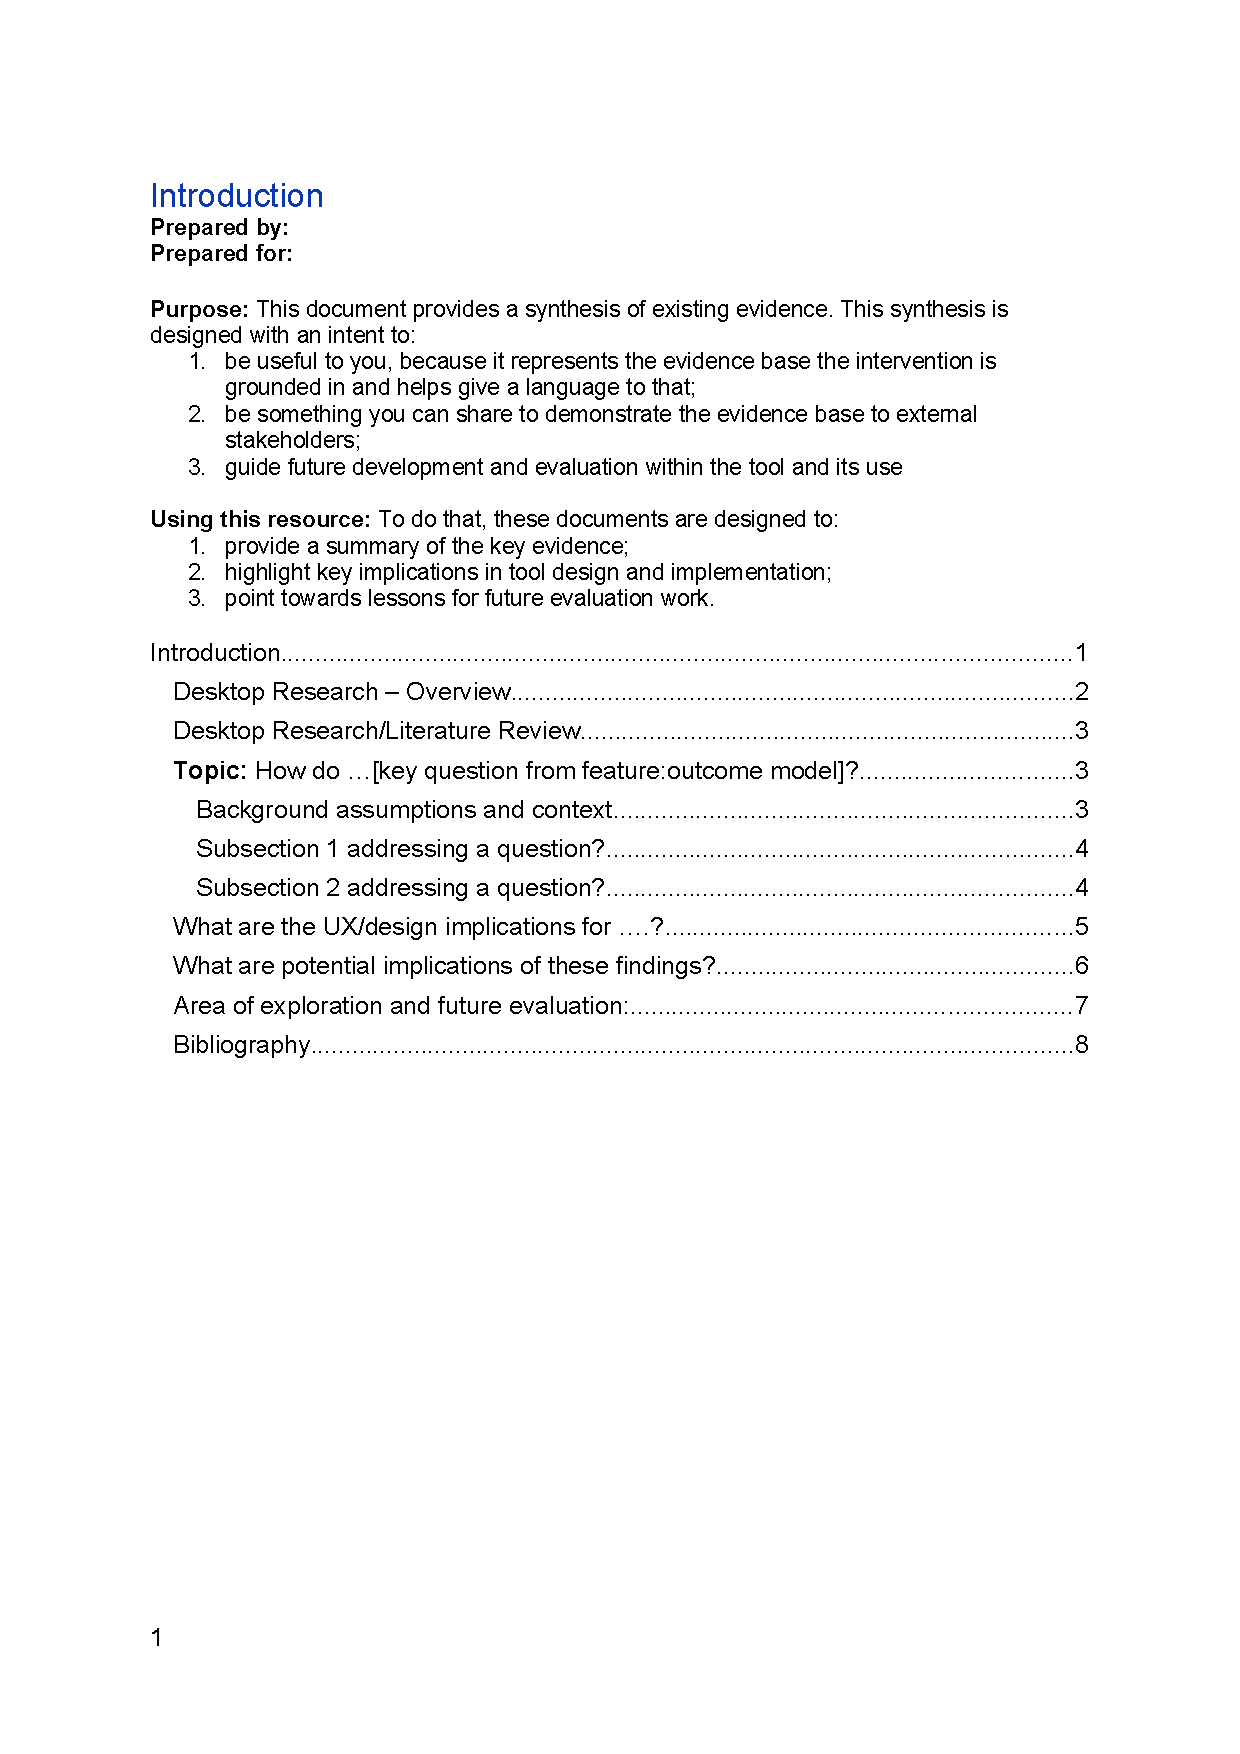
\includepdf[pages=-,noautoscale, width=205mm, height = 240mm, pagecommand={}]{data/04-synthesis/04-synthesis-checkins.pdf}\label{fig:synthesis-checkin}

\hypertarget{checkins-faq}{%
\subsection{Checkins FAQ}\label{checkins-faq}}

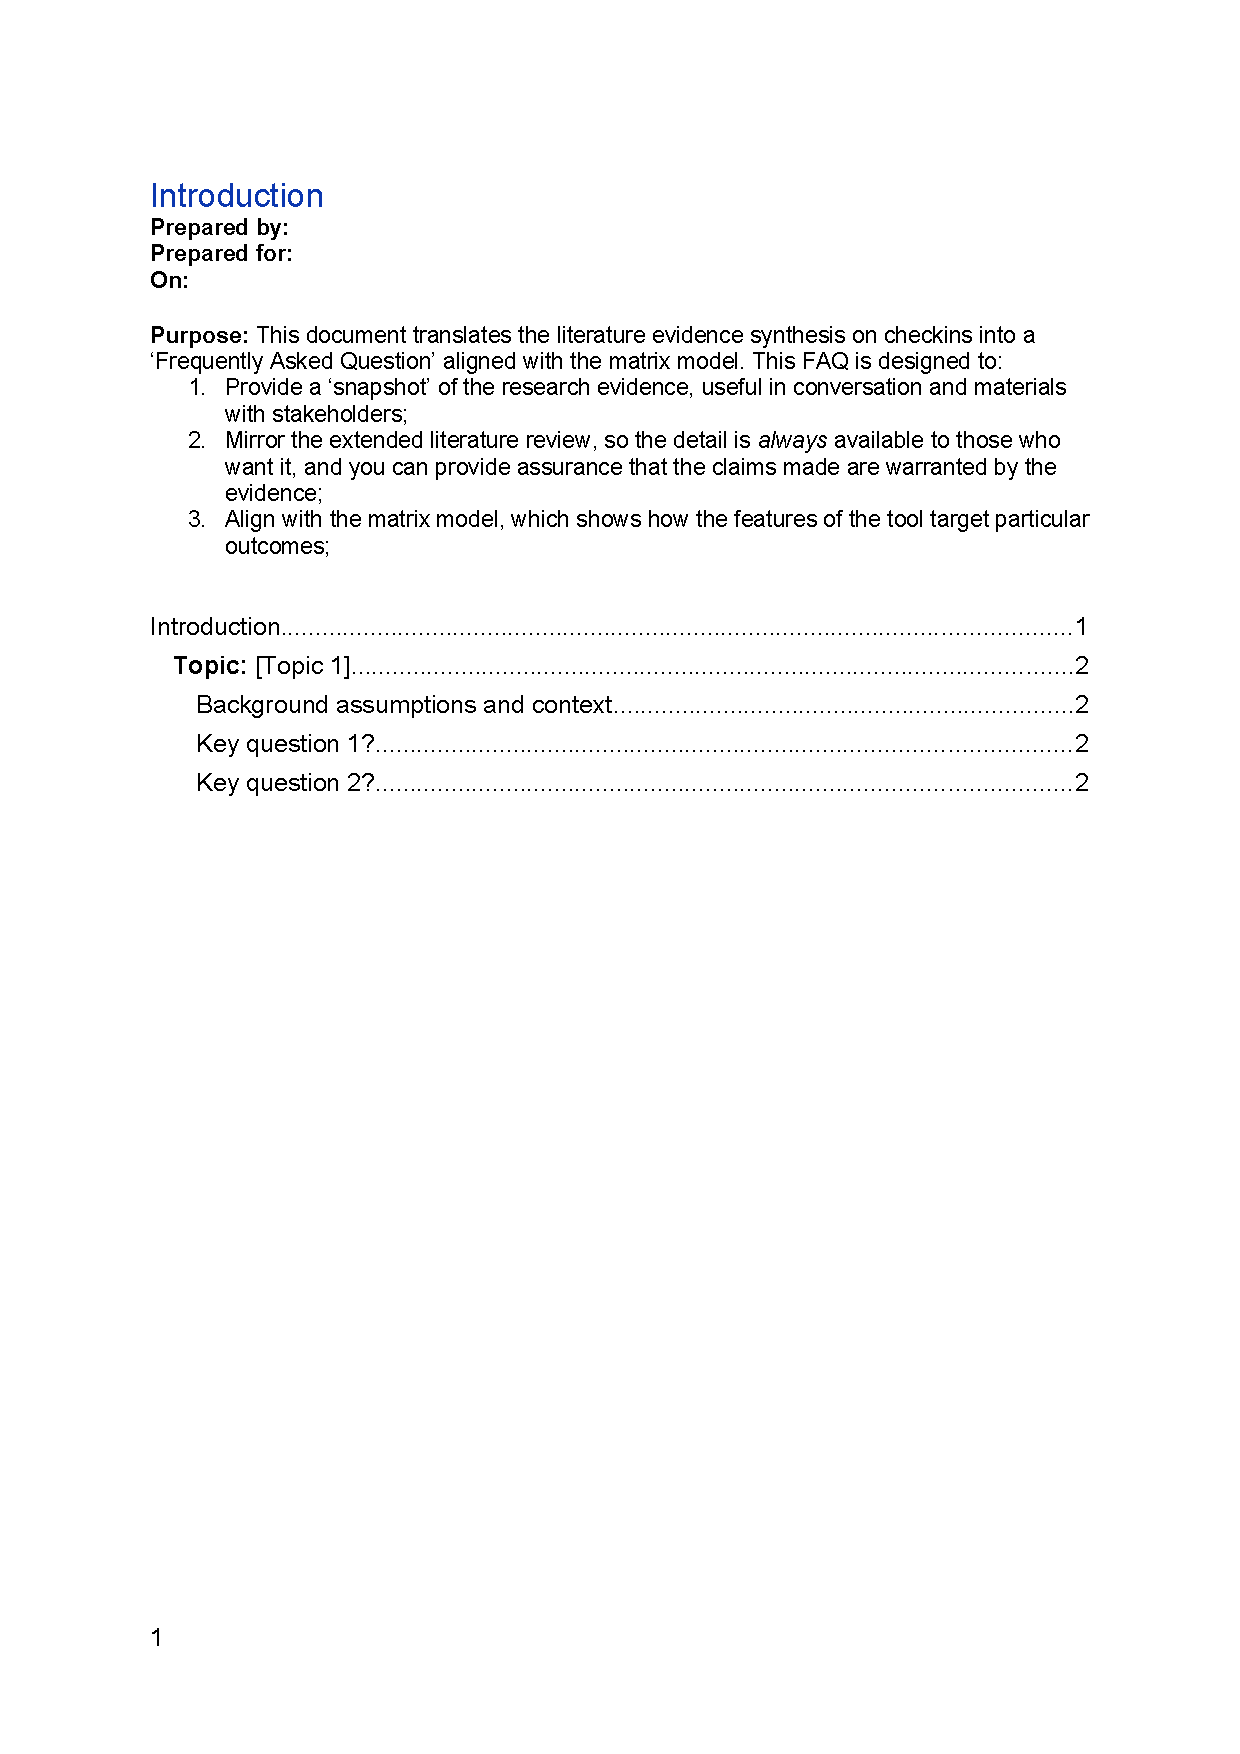
\includepdf[pages=-,noautoscale, width=205mm, height = 240mm, pagecommand={}]{data/04-synthesis/04-synthesis-checkins-FAQ.pdf}\label{fig:synthesis-checkin-faq}

\hypertarget{factors}{%
\chapter{An evidence informed tool: Identifying factors}\label{factors}}

\hypertarget{background}{%
\section{Background}\label{background}}

This section addresses the following questions in the model, through evidence synthesis, resource creation and mapping, and resources for stakeholders. Specifically, we analyse, evaluation of existing models of x and behavioural change, existing resources, and design research regarding \ldots{}

\begin{enumerate}
\def\labelenumi{\arabic{enumi}.}
\tightlist
\item
  .
\item
  .
\item
  .
\end{enumerate}

\hypertarget{factors-in-the-space}{%
\section{Factors in the space}\label{factors-in-the-space}}

\hypertarget{background-1}{%
\subsection{Background}\label{background-1}}

Work was undertaken to align with evidence-based models of x, to identify the key \emph{factors} that constitute x, and their relationship to y.

\hypertarget{document-1}{%
\subsection{Document 1}\label{document-1}}

Based on this initial mapping..

A document setting out models in the space.

\hypertarget{intervention-design}{%
\section{intervention designs}\label{intervention-design}}

Document setting out models for intervention in the space.

\hypertarget{resource-mapping}{%
\subsection{Resource mapping}\label{resource-mapping}}

Documents mapping a range of existing external resources to the model in \ref{fig:mapping}.


\includepdf[pages=-,noautoscale, width=205mm, height = 240mm, pagecommand={}]{data/05-intervention-files/mapping2.pdf}\label{fig:mapping}


\includepdf[pages=-,noautoscale, width=205mm, height = 240mm, pagecommand={}]{data/05-intervention-files/mapping2.pdf}\label{fig:factors-pdf-demo}

\textbf{Inclusion criteria:}

\begin{itemize}
\tightlist
\item
  here
\item
  and here
\end{itemize}

\hypertarget{stakeholder-resources}{%
\section{Stakeholder resources}\label{stakeholder-resources}}

Based on the research, two key stakeholder-oriented resources were created:

\begin{enumerate}
\def\labelenumi{\arabic{enumi}.}
\tightlist
\item
  A powerpoint resource, intended to introduce factors \ldots{}
\item
  A guide which provides an overview of the background to x and its use in classes\ldots{}
\end{enumerate}

These can be augmented with the resource mapping\ldots{}

\hypertarget{users}{%
\chapter{User research}\label{users}}

\hypertarget{background-2}{%
\section{Background}\label{background-2}}

A scenario based approach was used to focus the research, and engage with stakeholders via interviews. These scenarios help us to focus in on key issues that arise (1) out of the existing evidence base, and (2) in practice. The scenarios are intended to:

\begin{enumerate}
\def\labelenumi{\arabic{enumi}.}
\tightlist
\item
  help map out how x `works' to achieve its impact,
\item
  to explore this with teachers, to understand how they would use the tool, what existing resources they make use of that could be incorporated into the tool, and where there are gaps in the tool
\item
  in a second round of interviews, to revisit the scenarios once support resources are piloted, to evaluate their potential
\end{enumerate}

In addition to scenarios, the teacher interviews made use of other open questions, and a brief survey.

A feature of the design approach adopted is that the emergence of the literature, and its mapping to a change model for the tool/implementation should be considered in the design and execution of subsequent phases (which may also indicate need to review further literature, or/and revise the model). As such, the exact nature of the scenarios selected for semi-structured interview was iterated, and shaped to address the particular foci of the emerging work. This process was informed by both the existing tool and its user journey(s), and literature including work using or describing scenarios, and research using other methods such as survey instruments to probe particular drivers of change.

\hypertarget{research-ethics-in-australia}{%
\subsection{Research ethics in Australia}\label{research-ethics-in-australia}}

\begin{itemize}
\tightlist
\item
  Ethics required for any research involving human participation, this is done at a university level
\item
  The process sets out what we'll do and why, who will participate, and how we'll recruit them
\item
  The UTS research team sought and gained HREC approval
\end{itemize}

\hypertarget{approach}{%
\section{Approach}\label{approach}}

Participants were invited to\ldots{}

The interviews were recorded via video conferencing software, and transcribed in part, with prior permission of the participants.

Scenarios were developed to capture the user experience, particularly with reference to the key issues and questions identified in the model. This allowed us to clearly link the implicit theory in the matrix, the evidence synthesis, any open questions, and the user experience and needs together, to triangulate and identify key areas of focus.

\emph{Phase 1 Interviews}

Semi-structured interviews via video conferencing software\ldots{}

\emph{Phase 2 Interviews}

These semi-structured interviews again took place via video conferencing software \ldots{}

\hypertarget{removed-here}{%
\section{Removed here}\label{removed-here}}

Both sets of scenarios removed.

A round 1 and round 2 report were developed, with a powerpoint (not included here).

\hypertarget{proposed-directions}{%
\chapter{Proposed Directions}\label{proposed-directions}}

A set of recommendations are presented below, drawing on the evidence synthesised, analysis of other tools and platforms available, expert input and practitioner input.

These recommendations are intended to situate x's connection to the evidence base at present, possible gaps/misalignment with this evidence, and opportunities to align and contribute to the evidence base.

\hypertarget{assumptions}{%
\section{Assumptions}\label{assumptions}}

The literature has a number of potential implications for x development. However it is important to remember that any recommendations from literature are based on the specific aims and theories of change being evaluated and investigated in that literature. x adopts a different model to much of this literature, and therefore the recommendations are not directly transferable.

We have tried to provide these recommendations in a fairly agnostic form, so they are not contingent on specific implementation (and prioritisation), which is largely the remit of x

\hypertarget{recommendations}{%
\section{Recommendations}\label{recommendations}}

\begin{enumerate}
\def\labelenumi{\arabic{enumi}.}
\tightlist
\item
\end{enumerate}

\hypertarget{key-resources-collated-from-elsewhere-for-reference-here}{%
\section{Key resources (collated from elsewhere, for reference here)}\label{key-resources-collated-from-elsewhere-for-reference-here}}

\hypertarget{doc-1}{%
\subsection{doc 1}\label{doc-1}}

Headline issues from the range of docs (not covered in the evidence synthesis summaries).

\hypertarget{key-issues-from-evidence-synthesis}{%
\subsection{Key issues from evidence synthesis}\label{key-issues-from-evidence-synthesis}}

You'll see below that these recommendations (key issues largely highlighted in red) are reflected across the teacher work and wider analysis of the evidence.

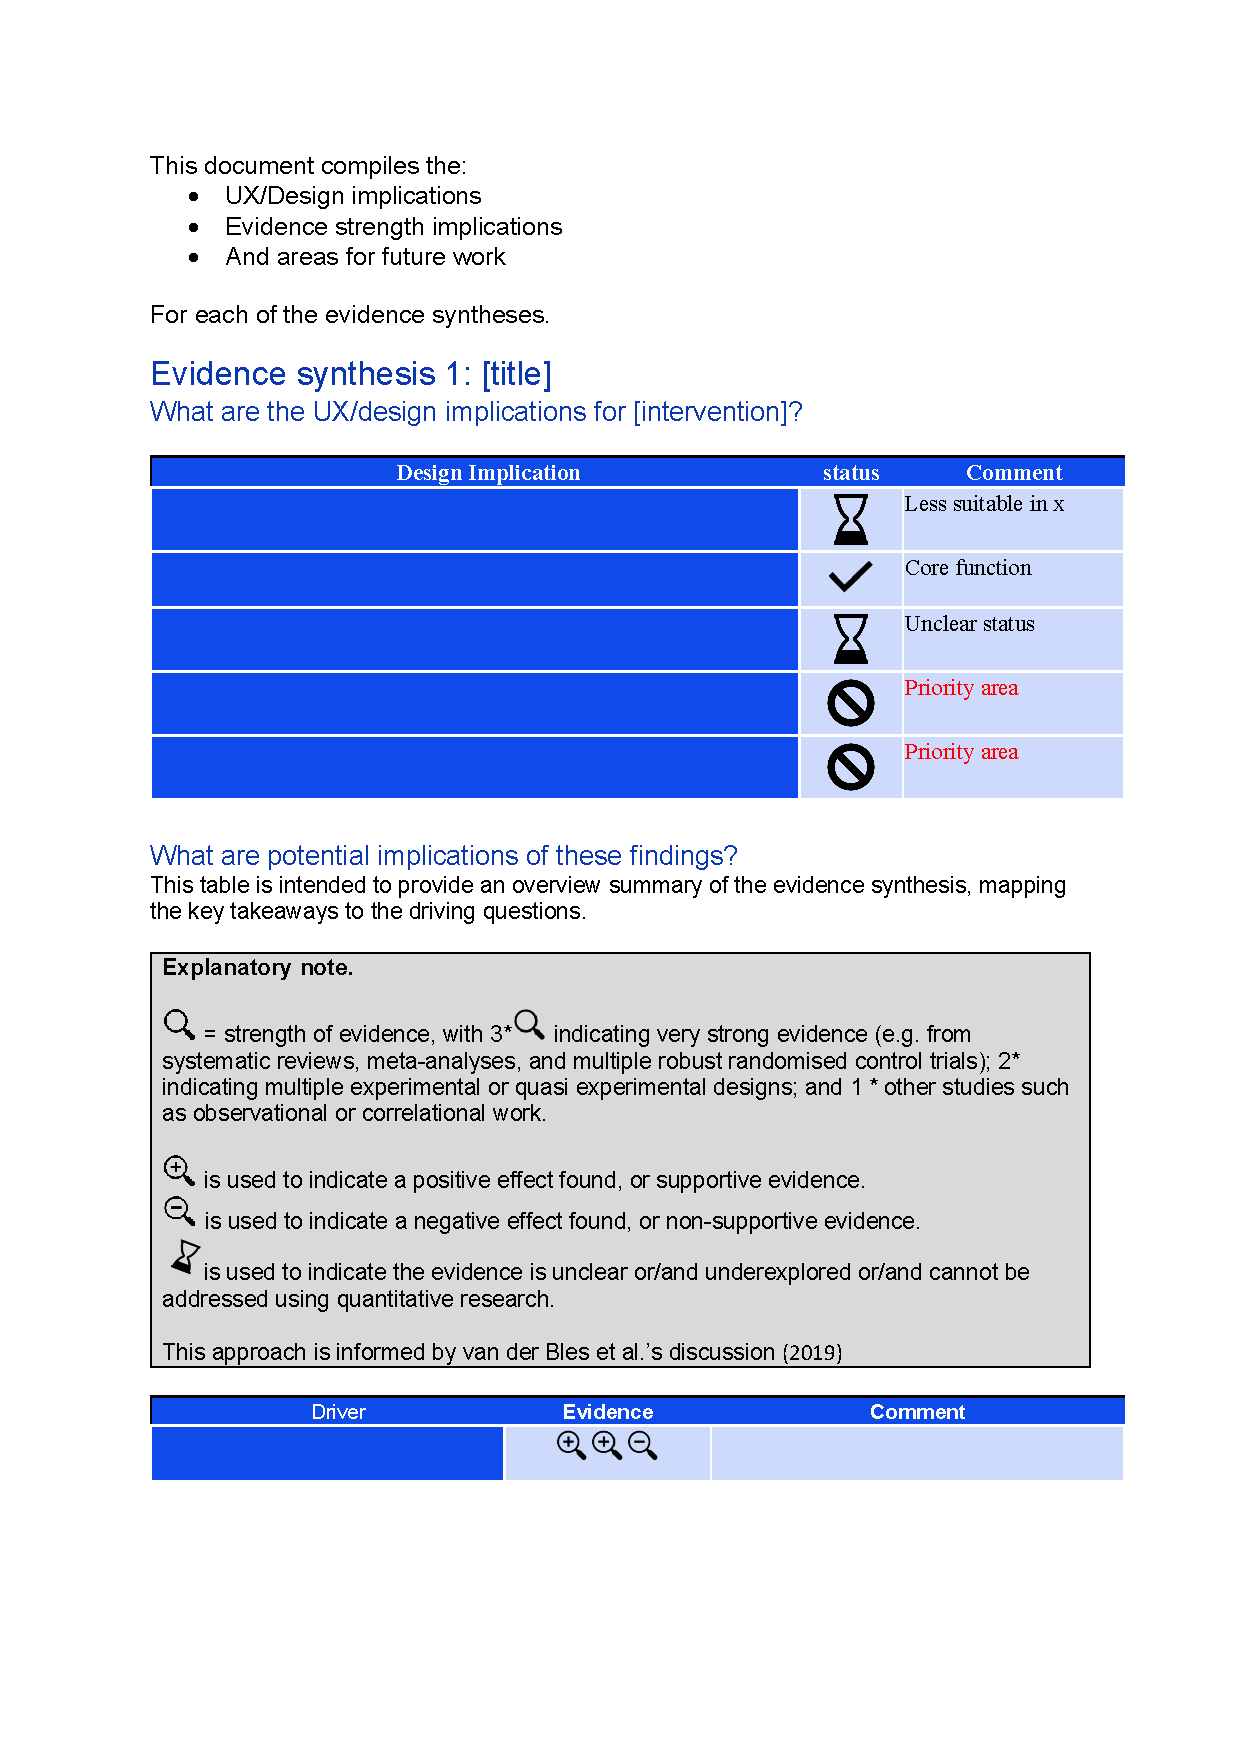
\includepdf[pages=-,noautoscale, width=205mm, height = 240mm, pagecommand={}]{data/07-recommendations/01-recommendations.pdf}\label{fig:synthesis-recommendations}

\hypertarget{references-used}{%
\chapter{References used}\label{references-used}}

\hypertarget{refs}{}
\begin{CSLReferences}{1}{0}
\leavevmode\vadjust pre{\hypertarget{ref-R-rmarkdown}{}}%
Allaire, JJ, Yihui Xie, Jonathan McPherson, Javier Luraschi, Kevin Ushey, Aron Atkins, Hadley Wickham, Joe Cheng, Winston Chang, and Richard Iannone. 2022. \emph{Rmarkdown: Dynamic Documents for r}. \url{https://CRAN.R-project.org/package=rmarkdown}.

\leavevmode\vadjust pre{\hypertarget{ref-bakkerMentalHealthSmartphone2016}{}}%
Bakker, David, Nikolaos Kazantzis, Debra Rickwood, and Nikki Rickard. 2016. {``Mental {Health Smartphone Apps}: {Review} and {Evidence-Based Recommendations} for {Future Developments}.''} \emph{JMIR Mental Health} 3 (1): e4984. \url{https://doi.org/10.2196/mental.4984}.

\leavevmode\vadjust pre{\hypertarget{ref-bakkerEngagementMobilePhone2018a}{}}%
Bakker, David, and Nikki Rickard. 2018. {``Engagement in Mobile Phone App for Self-Monitoring of Emotional Wellbeing Predicts Changes in Mental Health: {MoodPrism}.''} \emph{Journal of Affective Disorders} 227 (February): 432--42. \url{https://doi.org/10.1016/j.jad.2017.11.016}.

\leavevmode\vadjust pre{\hypertarget{ref-R-base}{}}%
R Core Team. 2021. \emph{R: A Language and Environment for Statistical Computing}. Vienna, Austria: R Foundation for Statistical Computing. \url{https://www.R-project.org/}.

\leavevmode\vadjust pre{\hypertarget{ref-knitr2014}{}}%
Xie, Yihui. 2014. {``Knitr: A Comprehensive Tool for Reproducible Research in {R}.''} In \emph{Implementing Reproducible Computational Research}, edited by Victoria Stodden, Friedrich Leisch, and Roger D. Peng. Chapman; Hall/CRC. \url{http://www.crcpress.com/product/isbn/9781466561595}.

\leavevmode\vadjust pre{\hypertarget{ref-knitr2015}{}}%
---------. 2015. \emph{Dynamic Documents with {R} and Knitr}. 2nd ed. Boca Raton, Florida: Chapman; Hall/CRC. \url{https://yihui.org/knitr/}.

\leavevmode\vadjust pre{\hypertarget{ref-bookdown2016}{}}%
---------. 2016. \emph{Bookdown: Authoring Books and Technical Documents with {R} Markdown}. Boca Raton, Florida: Chapman; Hall/CRC. \url{https://bookdown.org/yihui/bookdown}.

\leavevmode\vadjust pre{\hypertarget{ref-R-bookdown}{}}%
---------. 2022a. \emph{Bookdown: Authoring Books and Technical Documents with r Markdown}. \url{https://CRAN.R-project.org/package=bookdown}.

\leavevmode\vadjust pre{\hypertarget{ref-R-knitr}{}}%
---------. 2022b. \emph{Knitr: A General-Purpose Package for Dynamic Report Generation in r}. \url{https://yihui.org/knitr/}.

\leavevmode\vadjust pre{\hypertarget{ref-rmarkdown2018}{}}%
Xie, Yihui, J. J. Allaire, and Garrett Grolemund. 2018. \emph{R Markdown: The Definitive Guide}. Boca Raton, Florida: Chapman; Hall/CRC. \url{https://bookdown.org/yihui/rmarkdown}.

\leavevmode\vadjust pre{\hypertarget{ref-rmarkdown2020}{}}%
Xie, Yihui, Christophe Dervieux, and Emily Riederer. 2020. \emph{R Markdown Cookbook}. Boca Raton, Florida: Chapman; Hall/CRC. \url{https://bookdown.org/yihui/rmarkdown-cookbook}.

\end{CSLReferences}

\end{document}
